Here we study the jet energy scale (JES) and jet energy resolution (JER)
systematic uncertainties for the string resonances. 
The JES configuration used is StrongReduction JES; this configuration
has three nuisance parameter groups.
The JER configuration used is SimpleJER; this configuration has seven
nuisance parameter groups.
In examining the affects of these uncertainties, we consider the signal
samples as normalised template shapes. 

The affect of JES on the signal samples is studied by considering the
shift in the mean of the distribution for each JES nuisance parameter
group.
The affect of JER on the signal samples is studied by considering the
change in the RMS (or standard deviation) of the distribution for each
JER nuisance parameter group
We have also parameterised the signal shifts and width changes by
fitting a gaussian function to a few of the most significant bins around
the maximum value of the distribution. 
Similar results are obtain to just looking at the shift in the mean
distribution and the change in the RMS of the distribution.
Since this analysis not used in the calculation of the affects of
systematic uncertainties on the limits, we simplify by just
consider the mean and RMS of the distributions. 

Figure~\ref{fig2} shows an example for the $\Ms = 8$~TeV signal sample
and the JES GroupedNP\_3 group.
This represents the histogram of one of the systematics that are used in
the limit calculation.
The GroupedNP\_3 group was found to give the biggest shift in the signal
mean.
By looking at all the signal samples, we note that the reconstructed
signal peak is shifted low relative to the generated peak by $\sim
0.92\Ms$, even before accounting for the JES or JER systematic
uncertainties. 

\begin{figure}[htb]
\begin{center}
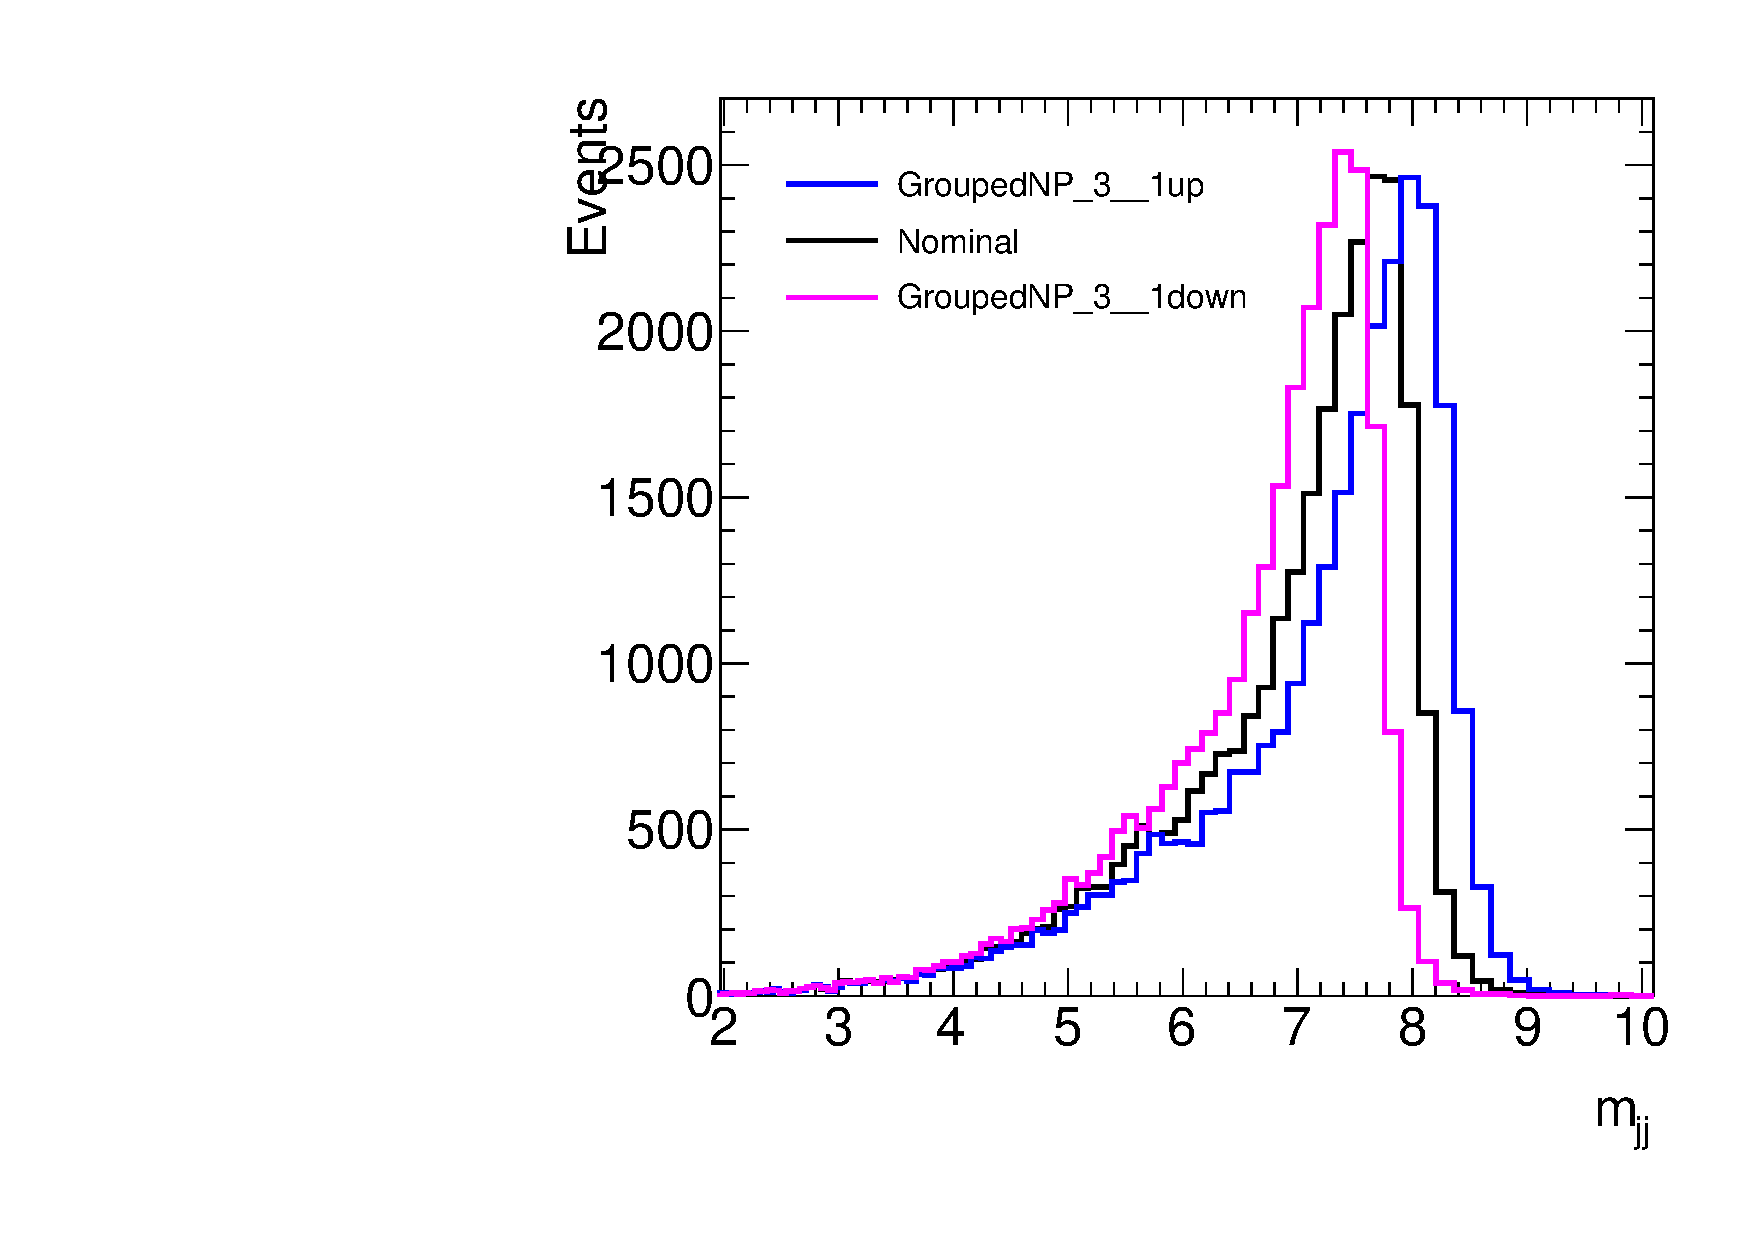
\includegraphics[width=0.7\linewidth]{figures/strings/JES_shift}
\end{center}
\caption{\mjj distribution for the $\Ms = 8$~TeV string sample (nominal).
Also shown are the distributions using the jet energy scale
GroupedNP\_3 one standard deviation up and down systematic uncertainties.}
\label{fig2}
\end{figure}

Figure~\ref{fig3} shows the relative shift in the mean of the \mjj
distribution due to the JES uncertainty and the relative change in RMS
of the \mjj distribution due to the JER uncertainty. 
Although all the nuisance parameter groups are used independently in the
limit calculations and we have look at each individually, for
illustrative purposes here we add all three JES mean shifts in quadrature
and all seven JER resolutions differences in quadrature. 

\begin{figure}[htb]
\begin{center}
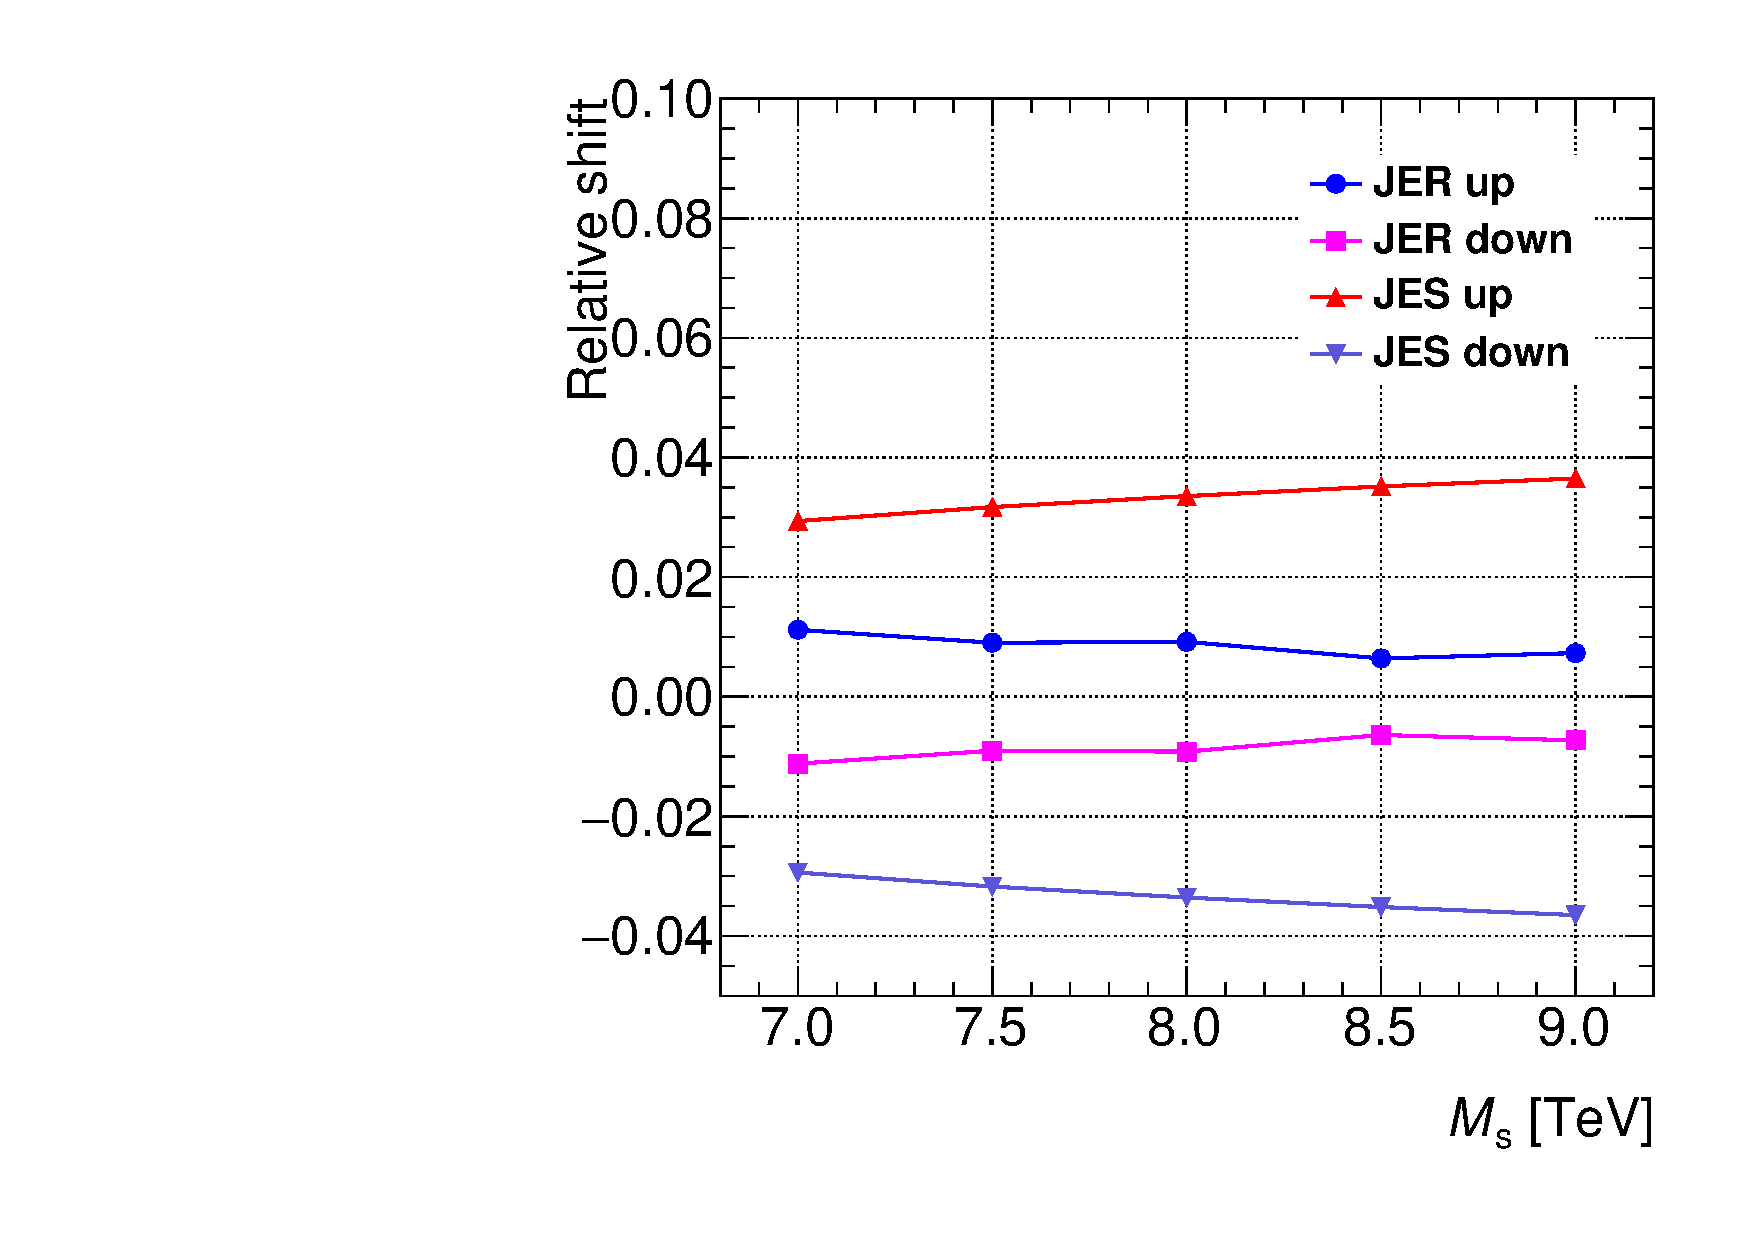
\includegraphics[width=0.7\linewidth]{figures/strings/JES_JER}
\end{center}
\caption{Relative shift in the mean of the \mjj distributions for each
string sample due to jet energy scale uncertainty, and relative change
in the RMS of the \mjj distributions for each string sample due to the
jet energy resolution uncertainty.
The changes due to each nuisance parameter group are added in
quadrature.}
\label{fig3}
\end{figure}

The change in signal acceptance due to JES and JER uncertainties are
added in quadrature and determined to be less than 0.06\%. 
We ignore this small uncertainty when using values for the signal
acceptance.
The change in mean of the signal distributions due to the JES uncertainty is
less than 4\%; it is dominated by GroupedNP\_3. 
The change in RMS of the signal distributions due to the JER uncertainty
is less than 1.2\%.
This uncertainty is most significant for the lowest \Ms signal sample and
each of the seven values that are added in quadrature do not have a
dominate component.


